\chapter{Design of the Solution}
\label{ch:design}

\begin{chapterquote}{Ludwig Wittgenstein}
	The limits of my language mean the limits of my world.
\end{chapterquote}

The model was implemented in Keras, a high-level neural networks library written in Python. It can run on top of either TensorFlow or Theano and with CPU or GPU. It supports recurrent networks, and arbitrary connectivity schemes including multi-input and multi-output training. 

\section{Text representation}

In this section we explain how characters are mapped to an adequate representation that the network can understand. Training the RNN on many shorter sequences is just as effective as training the whole string at once. Also this is a better choice since to compute the exact gradient of the log probability of the training set, the RNN needs to process the entire training set sequentially and store the hidden state sequence to apply BTT. This task is infeasible due to the size of the training sets as well as unnecessary\cite{sutskever2011generating}.

 Therefore, to represent the text of length N containing M different characters, we focus on specific text windows of length F that we check every step size S. Then, the number of sequences is given by the integer division: $NbSq=(N-F)/S$. 

For example, if we have the phrase of Ludwig Wittgenstein "The limits of my language are the limits of my world" we have a text of length $N=52$ and $M=19$ different characters. If we set $F=4$ and $S=2$ we have 24 sequences whose target is its next character as showed in table \ref{tab:seqch}.

\begin{table}{}

\begin{tabular}{c c}
\textbf{Phrase: }&The limits of my language are the limits of my world \\
\end{tabular}
\begin{tabular}{c c c c c c c c c c c c c c c c c c c c c}
\textbf{No.}&0&1&2&3&4&5&6&7&8&9&10&11&12&13&14&15&16&17&18\\
\textbf{Characters:}& " "& T& a& d& e& f& g& h& i& l& m& n& o& r& s& t& u& w& y\\https://preview.overleaf.com/public/dvwgvfjpjgzz/images/9c4e1806cd4b1e85cd91e9f211717f2c0d977d8c.jpeg
\end{tabular}
\caption{Number of Characters}
\end{table}https://preview.overleaf.com/public/dvwgvfjpjgzz/images/9c4e1806cd4b1e85cd91e9f211717f2c0d977d8c.jpeg
\begin{table}{}
\begin{tabular}{c c c c c c c c c c c c c c}
\textbf{Sequence:} &0&1&2 & 3 &4&5&6&7&8&9&10&11\\
\textbf{Chars:} &The &e li&limi&mits&ts o& of &f my&my l& lan&angu&guag&age\\ 
\textbf{Next character: }&l&m&t&" "&f&m&" "&a&g&a&e&a\\
\textbf{Sequence:} &12&13&14&15&16&17&18&19&20&21&22&23\\
\textbf{Chars:} &e ar&are &e th&the &e li&limi&mits&ts o& of &f my&my w& wor\\
\textbf{Next character: }&e&t&e&l&m&t&" "&f&m&" "&o&l\\
\end{tabular}

\caption{Sequences of Characters}
\label{tab:seqch}

\end{table}


Next we have to use the one-of-K representation for each character in each sequence. Since the number of text classes is the number of different characters for each sequence $(ns,f);  ns \in NbSq; f \in F $, we need a vector of size $M$ where every element is a zero except for the number of element that corresponds to the character. For example, if $ns=13$ and $f=1$ the character is 'a' and therefore its one-of-K representation is: $[0,0,1,0,0,0,0,0,0,0,0,0,0,0,0,0,0,0,0,]$. 
Now we have a matrix of dimensions: $S$x$F$x$M$ that represents the text of length $N$. This matrix is the input of the network. Conversely, the target next characters are mapped to the one-of-K representation, too. This will model a $NbSq x M$ matrix. 
In this work we used sequences of length $F=250$ as in \cite{sutskever2011generating}

\section{Network Architecture}

The model has an input, a hidden and an output layer. The input layer has the same number as the total of sequences $(NbSq)$. Each input is of dimensions $FxM$. The network has one single hidden layer with 1000 LSTM units as suggested in \cite{graves2013generating}.The LSTM has a drop out of 0.5 implemented  in both, recurrent and non-recurrent connections as described in \cite{gal2015theoretically}. 

Finally, because this is a classification problem we use a fully connected output layer with the same number of neurons as unique characters ($M$). It uses the softmax function as activation function to make predictions for each of the classes and the cross-entropy function as loss function. The network implements the  ADAM SGD optimizer in order to adapt the learning rate dynamically as the data is sparse. 

The next character is then the one with the greatest probability that is computed at the last step. The network scheme is showed in Fig.\ref{fig:netarch}  Where the $x_{i}$'s are the $M$ input sequences and $x_o$ is the predicted next character. Of course, $x_0$ needs to be translated from one-of-K representation to character representation at the end of the process.

\begin{figure}[h]
\centering
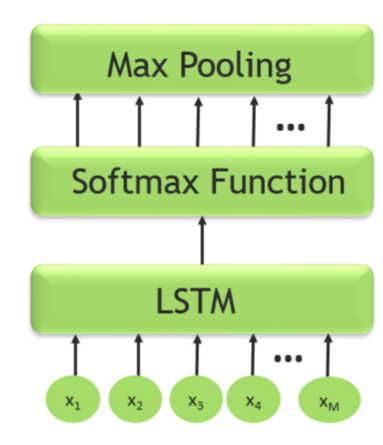
\includegraphics[width=6cm,height=7cm]{arquitectura.PNG}
\caption{Network Architecture}
\label{fig:netarch}
\end{figure}























